% Style reference: Overleaf "清华大学中文Beamer 模板" by 赵宗义,
% derived from the unofficial Tsinghua Beamer template, CC BY 4.0.
% This deck recreates the academic minimalist purple/white style locally
% without depending on missing external logo/theme assets.
\documentclass[aspectratio=43,10pt]{beamer}

\usepackage{ctex}
\usepackage{fontspec}
\usepackage{amsmath,amssymb}
\usepackage{booktabs}
\usepackage{tabularx}
\usepackage{tikz}
\usepackage{graphicx}
\usetikzlibrary{arrows.meta,positioning,calc}

\setmainfont{Helvetica}
\setsansfont{Helvetica}
\setCJKmainfont{Songti SC}
\setCJKsansfont{Songti SC}

\graphicspath{{fig/}}

\definecolor{thuPurple}{HTML}{5E2B83}
\definecolor{thuLight}{HTML}{EFEAF5}
\definecolor{ink}{HTML}{1F1F24}
\definecolor{muted}{HTML}{666A73}
\definecolor{accent}{HTML}{7A4AA0}
\definecolor{softBlue}{HTML}{E9F0F5}

\setbeamersize{text margin left=0.70cm,text margin right=0.70cm}
\setbeamercolor{normal text}{fg=ink,bg=white}
\setbeamercolor{structure}{fg=thuPurple}
\setbeamercolor{alerted text}{fg=thuPurple}
\setbeamerfont{frametitle}{size=\LARGE,series=\normalfont}
\setbeamerfont{title}{size=\Large,series=\normalfont}
\setbeamerfont{subtitle}{size=\normalsize}
\setbeamertemplate{navigation symbols}{}
\setbeamertemplate{itemize item}{\color{thuPurple}$\bullet$}
\setbeamertemplate{itemize subitem}{\color{thuPurple}\scriptsize$\blacktriangleright$}
\setbeamertemplate{enumerate item}{\color{thuPurple}\insertenumlabel.}

\setbeamertemplate{frametitle}{%
  \vspace{0.18cm}
  \begin{tikzpicture}[remember picture,overlay]
    \fill[thuPurple] (current page.north west) --
      ([xshift=3.25cm,yshift=-0.24cm]current page.north west) --
      ([yshift=-0.44cm]current page.north west) -- cycle;
    \draw[thuPurple,line width=0.35pt]
      ([xshift=10.85cm,yshift=-0.70cm]current page.north west) --
      ([xshift=12.78cm,yshift=-0.70cm]current page.north west);
    \node[anchor=north east,text=ink,font=\large]
      at ([xshift=-0.45cm,yshift=-0.20cm]current page.north east)
      {\insertframenumber};
  \end{tikzpicture}
  \hspace{-0.15cm}\insertframetitle\par
  \vspace{0.54cm}
}

\setbeamertemplate{footline}{%
  \begin{tikzpicture}[remember picture,overlay]
    \fill[thuPurple] (current page.south west) rectangle
      ([yshift=0.33cm]current page.south east);
  \end{tikzpicture}
  \vspace{0.33cm}
}

\newcommand{\hl}[1]{\textcolor{thuPurple}{\textbf{#1}}}
\newcommand{\smallgray}[1]{{\scriptsize\textcolor{muted}{#1}}}
\newcommand{\tightitems}{\setlength{\itemsep}{0.35em}}
\newcommand{\framecite}[1]{\vfill{\scriptsize\textcolor{muted}{#1}}}

\title{AtomWorld-Mirror: Macro-Step World Modeling of Critical Evolution Backbones for Materials Dynamics}
\subtitle{}
\author{%
  \normalfont
  \textbf{Ziming Pan}$^{1,2,*}$ \quad
  \textbf{Ruge Zhang}$^{1,4,5,*}$ \quad
  \textbf{Haozhi Han}$^{1,3}$\\
  \textbf{Yifeng Chen}$^{3}$ \quad
  \textbf{Yunquan Zhang}$^{4}$ \quad
  \textbf{Ting Cao}$^{1}$\\
  \textbf{Yunxin Liu}$^{1}$ \quad
  \textbf{Kun Li}$^{1,\dagger}$\\[0.18cm]
  {\scriptsize $^1$Institute for AI Industry Research (AIR), Tsinghua University, Beijing, China}\\
  {\scriptsize $^2$Yonsei University, Seoul, Republic of Korea}\\
  {\scriptsize $^3$School of Computer Science, Peking University, Beijing, China}\\
  {\scriptsize $^4$Institute of Computing Technology, Chinese Academy of Sciences, Beijing, China}\\
  {\scriptsize $^5$School of Computer Science and Technology, University of Chinese Academy of Sciences}\\
  {\scriptsize Beijing, China}\\
  {\scriptsize $^*$Equal contribution. \quad $^\dagger$Corresponding author. \quad \texttt{likun@air.tsinghua.edu.cn}}
}
\institute{}
\date{\today}

\begin{document}

{\setbeamertemplate{footline}{}
\begin{frame}[plain]
  \begin{center}
    \vspace{0.70cm}
    {\color{thuPurple}\Large AtomWorld-Mirror:\\[0.12cm]
    Macro-Step World Modeling of Critical Evolution Backbones\\
    for Materials Dynamics\par}
    \vspace{0.48cm}
    {\small \insertauthor\par}
  \end{center}
\end{frame}
}

\begin{frame}{原子模拟：从微观规则推演材料演化}
  \small
  \begin{columns}[T,onlytextwidth]
    \begin{column}{0.44\textwidth}
      \textbf{基本对象}
      \begin{itemize}
        \tightitems
        \item 状态是原子构型、局部环境和物理时钟。
        \item 目标是从 microscopic rules 推演 diffusion、aging、defect evolution 等长时程行为。
        \item 轨迹由大量 local updates 组成。
      \end{itemize}
      \vspace{0.35cm}
      \hl{关键问题：}如何从局部演化得到长期结构进展。
    \end{column}
    \begin{column}{0.52\textwidth}
      \textbf{常见方法与成本来源}
      \begin{itemize}
        \tightitems
        \item Molecular dynamics：显式短时间步；长时程需要海量 steps。
        \item KMC / Gillespie：逐个微事件推进；每步更新局部环境、速率和物理时钟。
        \item Monte Carlo / coarse-graining：降低采样或自由度成本，但仍要遍历大量状态。
        \item learned potentials / graph simulators：降低局部计算成本，但通常仍沿 dense rollout 推进。
      \end{itemize}
      \vspace{0.25cm}
      \smallgray{为什么贵：大体系 × 长时间尺度 × 每步物理计算；关键结构变化又很稀疏，预算常先耗在低影响中间态。}
    \end{column}
  \end{columns}
\end{frame}

\begin{frame}{逐步推进会混合两类变化}
  \begin{columns}[T,onlytextwidth]
    \begin{column}{0.47\textwidth}
      \textbf{低影响中间态}
      \begin{itemize}
        \tightitems
        \item 短暂局部波动
        \item 对未来结构进展影响弱
        \item 仍然触发状态更新、速率计算和时钟推进
      \end{itemize}
    \end{column}
    \begin{column}{0.47\textwidth}
      \textbf{持续结构进展}
      \begin{itemize}
        \tightitems
        \item 稀疏但会累积
        \item 约束后续材料演化方向
        \item 应成为长时程建模的保留对象
      \end{itemize}
    \end{column}
  \end{columns}
  \vspace{0.75cm}
  \begin{center}
    \Large \hl{传统逐微事件或逐时间步表述，对不同状态变化近似一视同仁。}
  \end{center}
\end{frame}

\begin{frame}{Figure 1：关键结构变化稀疏且随机}
  \begin{columns}[T,onlytextwidth]
    \begin{column}{0.43\textwidth}
      \begin{itemize}
        \tightitems
        \item 很多低影响局部更新消耗 replay budget。
        \item 真正关键的结构变化只稀疏出现。
        \item Figure 1 统计 teacher Cu--Fe aging trajectories。
        \item Cu-vacancy key events 在 1000-step budget 中分布稀疏且随机。
      \end{itemize}
    \end{column}
    \begin{column}{0.53\textwidth}
      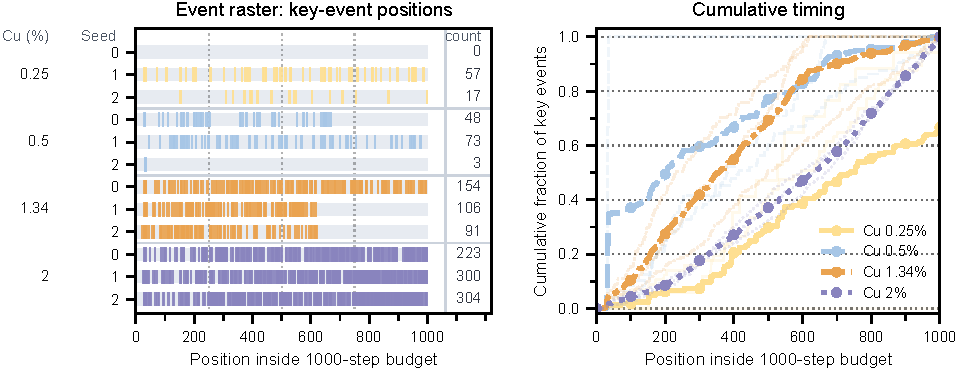
\includegraphics[width=\linewidth]{fig1_key_evolution_budget_randomness.pdf}
      \smallgray{同一 1000-step budget 内，key events 的位置随 seed 和浓度改变。}
    \end{column}
  \end{columns}
\end{frame}

\begin{frame}{Related work：轨迹加速 vs. 方向选择}
  \small
  \begin{columns}[T,onlytextwidth]
    \begin{column}{0.31\textwidth}
      \textbf{Coarse-grained MD\\force matching}
      \begin{itemize}
        \tightitems
        \item fine atoms / interactions
        \item \(\rightarrow\) coarse beads 或 effective potentials
        \item 降低连续动力学自由度
      \end{itemize}
    \end{column}
    \begin{column}{0.31\textwidth}
      \textbf{Coarse-grained KMC\\Monte Carlo}
      \begin{itemize}
        \tightitems
        \item microscopic cells / events / occupancies
        \item \(\rightarrow\) coarser units
        \item 降低事件数或状态数
      \end{itemize}
    \end{column}
    \begin{column}{0.31\textwidth}
      \textbf{MSM\\state lumping}
      \begin{itemize}
        \tightitems
        \item trajectory microstates
        \item \(\rightarrow\) metastable macrostates
        \item 学习 transition matrix
      \end{itemize}
    \end{column}
  \end{columns}
  \vspace{0.28cm}
  \begin{center}
    \begin{minipage}{0.91\linewidth}
      \small
      \hl{共同限制：}这些方法降低成本，但保留状态通常由粗粒变量、
      亚稳性或采样转移统计决定；它们不显式判断 evolution
      是否沿正确方向推进，也不回答哪些状态构成 critical evolution backbone。
      \smallgray{[59--62]}
    \end{minipage}
  \end{center}
  \vspace{0.18cm}
  {\scriptsize\textcolor{muted}{补充路线：learned potentials / graph simulators /
  physics-informed models 证明原子动力学可学习；rare-event 与 policy-guided search
  降低轨迹遍历成本，但通常仍面向 forces、dense states、local validation 或 reward-shaped search，
  而不是 reachable sparse macro edit with accumulated duration。\,[3,17,33,54,55,63--69]}}
\end{frame}

\begin{frame}{关键演化骨干：压缩低影响中间态}
  \begin{columns}[T,onlytextwidth]
    \begin{column}{0.48\textwidth}
      \[
      \mathcal{B}=(X_{n_0},X_{n_1},\ldots,X_{n_M}),\qquad M\ll N
      \]
      \begin{itemize}
        \tightitems
        \item 长时程建模不应保存所有低影响中间状态。
        \item backbone 保留承载持续结构进展的稀疏转换。
        \item 每个 macro transition 同时包含状态变化和累计物理时间。
        \item \(M\ll N\)：保留少数关键节点，而不是复现完整微事件序列。
      \end{itemize}
    \end{column}
    \begin{column}{0.48\textwidth}
      \begin{center}
      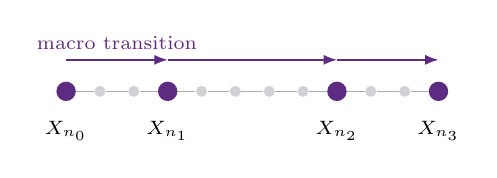
\begin{tikzpicture}[x=0.43cm,y=0.80cm]
        \foreach \i in {0,...,11} {
          \node[circle,fill=muted!30,minimum size=4pt,inner sep=0pt] (x\i) at (\i,0) {};
        }
        \foreach \i in {0,...,10} {
          \pgfmathtruncatemacro{\j}{\i+1}
          \draw[muted!55] (x\i) -- (x\j);
        }
        \foreach \i/\lab in {0/{\(X_{n_0}\)},3/{\(X_{n_1}\)},8/{\(X_{n_2}\)},11/{\(X_{n_3}\)}} {
          \node[circle,fill=thuPurple,minimum size=7pt,inner sep=0pt] at (\i,0) {};
          \node[below=0.25cm] at (\i,0) {\scriptsize \lab};
        }
        \draw[-{Latex[length=1.7mm]},thuPurple,line width=0.5pt] (0,0.50) -- node[above,font=\scriptsize] {macro transition} (3,0.50);
        \draw[-{Latex[length=1.7mm]},thuPurple,line width=0.5pt] (3,0.50) -- (8,0.50);
        \draw[-{Latex[length=1.7mm]},thuPurple,line width=0.5pt] (8,0.50) -- (11,0.50);
      \end{tikzpicture}
      \end{center}
      \vspace{0.5cm}
      \textbf{关键挑战：}\\
      不是事后压缩已生成轨迹，\\
      而是从当前构型向前选择下一个\\
      未来相关的 backbone state。
    \end{column}
  \end{columns}
\end{frame}

\begin{frame}{AtomWorld-Mirror：具有前瞻能力的 state-time world model}
  \begin{columns}[T,onlytextwidth]
    \begin{column}{0.48\textwidth}
      \textbf{模型含义}
      \begin{itemize}
        \tightitems
        \item AtomWorld：teacher simulator 暴露的原子演化世界。
        \item Mirror：学习原子演化的 latent counterpart。
        \item 它不复制微观轨迹本身，而是保留 future-relevant backbone 及其物理约束。
      \end{itemize}
    \end{column}
    \begin{column}{0.48\textwidth}
      \textbf{操作对象}
      \begin{itemize}
        \tightitems
        \item 从当前构型推断下一个 backbone transition。
        \item 解码为 physically reachable sparse edit。
        \item 预测该转移累计的 physical duration。
        \item 生成压缩但受物理约束的 state-time evolution backbone。
      \end{itemize}
    \end{column}
  \end{columns}
  \vspace{0.55cm}
  \begin{center}
    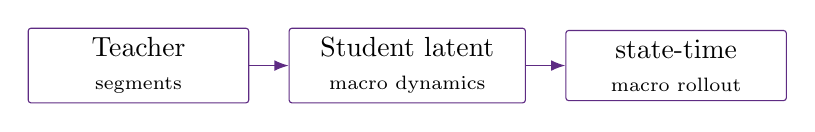
\begin{tikzpicture}[node distance=0.50cm]
      \node[draw=thuPurple,rounded corners=1pt,align=center,minimum width=2.8cm,minimum height=0.65cm] (a)
        {Teacher\\\scriptsize segments};
      \node[draw=thuPurple,rounded corners=1pt,align=center,minimum width=3.0cm,minimum height=0.65cm,right=of a] (b)
        {Student latent\\\scriptsize macro dynamics};
      \node[draw=thuPurple,rounded corners=1pt,align=center,minimum width=2.8cm,minimum height=0.65cm,right=of b] (c)
        {state-time\\\scriptsize macro rollout};
      \draw[-{Latex[length=1.8mm]},thuPurple] (a) -- (b);
      \draw[-{Latex[length=1.8mm]},thuPurple] (b) -- (c);
    \end{tikzpicture}
  \end{center}
\end{frame}

\begin{frame}{宏步任务：学习状态-时间宏转移}
  \begin{columns}[T,onlytextwidth]
    \begin{column}{0.48\textwidth}
      \textbf{输入}
      \begin{itemize}
        \tightitems
        \item 当前原子构型 \(X_t\)
        \item 选定的 macro horizon \(k\)
        \item teacher 给出的局部可达候选集合
      \end{itemize}
    \end{column}
    \begin{column}{0.48\textwidth}
      \textbf{输出}
      \begin{itemize}
        \tightitems
        \item 下一个骨干状态上的稀疏编辑
        \item 经过物理投影后的下一宏状态
        \item 该转移累计的物理时间
      \end{itemize}
    \end{column}
  \end{columns}
  \vspace{0.75cm}
  \begin{center}
    \begin{tikzpicture}[node distance=0.42cm]
      \node[draw=thuPurple,rounded corners=1pt,align=center,minimum width=2.3cm,minimum height=0.65cm] (x)
        {当前构型\\\scriptsize \(X_t\)};
      \node[draw=thuPurple,rounded corners=1pt,align=center,minimum width=2.6cm,minimum height=0.65cm,right=of x] (edit)
        {可达稀疏编辑\\\scriptsize sparse edit};
      \node[draw=thuPurple,rounded corners=1pt,align=center,minimum width=2.4cm,minimum height=0.65cm,right=of edit] (next)
        {下一宏状态\\\scriptsize \(X_{t+k}\)};
      \node[draw=muted,rounded corners=1pt,align=center,minimum width=2.0cm,minimum height=0.65cm,below=0.42cm of edit] (tau)
        {累计时间\\\scriptsize duration};
      \draw[-{Latex[length=1.8mm]},thuPurple] (x) -- (edit);
      \draw[-{Latex[length=1.8mm]},thuPurple] (edit) -- (next);
      \draw[-{Latex[length=1.5mm]},muted] (edit) -- (tau);
    \end{tikzpicture}
  \end{center}
  \framecite{目标不是预测完整微轨迹，而是学习可继续 rollout 的状态--时间宏步转移。}
\end{frame}

\begin{frame}{Teacher：提供连续时间监督}
  \begin{columns}[T,onlytextwidth]
    \begin{column}{0.48\textwidth}
      \textbf{微事件层面}
      \begin{itemize}
        \tightitems
        \item 局部速率决定下一次原子事件。
        \item 总速率决定等待时间尺度。
        \item 每个事件同时推进结构和物理时钟。
      \end{itemize}
    \end{column}
    \begin{column}{0.48\textwidth}
      \textbf{宏步监督层面}
      \begin{itemize}
        \tightitems
        \item teacher 短段给出起点、终点和实际触达区域。
        \item 路径摘要保留“怎样到达”的信息。
        \item \(\tau_{\mathrm{exp}}\) 是主时间标签；\(\tau_{\mathrm{real}}\) 用于随机时间诊断。
      \end{itemize}
    \end{column}
  \end{columns}
  \vspace{0.7cm}
  \begin{center}
    \large \hl{Teacher 的价值：局部事件合法 + 连续时间标签明确。}
  \end{center}
\end{frame}

\begin{frame}{Teacher supervision：宏步样本}
  \begin{columns}[T,onlytextwidth]
    \begin{column}{0.31\textwidth}
      \textbf{状态对象}
      \begin{itemize}
        \tightitems
        \item 当前构型
        \item teacher 终点
        \item 起点到终点的稀疏编辑
      \end{itemize}
    \end{column}
    \begin{column}{0.31\textwidth}
      \textbf{路径对象}
      \begin{itemize}
        \tightitems
        \item macro horizon
        \item microscopic path summary
        \item reachable candidate set
      \end{itemize}
    \end{column}
    \begin{column}{0.31\textwidth}
      \textbf{时间对象}
      \begin{itemize}
        \tightitems
        \item 累计期望时间
        \item 采样得到的真实等待时间
        \item 时间不确定性诊断
      \end{itemize}
    \end{column}
  \end{columns}
  \vspace{0.65cm}
  \begin{center}
    \large \hl{监督信号同时回答：哪里变了、怎么到达、用了多少物理时间。}
  \end{center}
\end{frame}

\begin{frame}{Student：macro world model}
  \begin{columns}[T,onlytextwidth]
    \begin{column}{0.42\textwidth}
      \begin{center}
      \begin{tikzpicture}[node distance=0.36cm,scale=0.72,transform shape]
        \node[draw=thuPurple,rounded corners=1pt,align=center,minimum width=2.45cm] (enc)
          {state encoder\\\scriptsize 当前构型表征};
        \node[draw=thuPurple,rounded corners=1pt,align=center,minimum width=2.35cm] (post) at ($(enc)+(-1.35,-1.05)$)
          {path posterior\\\tiny 训练期看 teacher path};
        \node[draw=thuPurple,rounded corners=1pt,align=center,minimum width=2.35cm] (prior) at ($(enc)+(1.35,-1.05)$)
          {path prior\\\tiny 推理期只看当前状态};
        \node[draw=thuPurple,rounded corners=1pt,align=center,minimum width=2.95cm,below=1.10cm of enc] (dyn)
          {macro dynamics\\\scriptsize 下一个 latent state};
        \node[draw=thuPurple,rounded corners=1pt,align=center,minimum width=2.95cm,below=0.42cm of dyn] (dec)
          {edit-duration decoder\\\scriptsize 编辑 + 时间 + reward};
        \draw[-{Latex[length=1.6mm]},muted] (enc) -- (post);
        \draw[-{Latex[length=1.6mm]},muted] (enc) -- (prior);
        \draw[-{Latex[length=1.6mm]},muted] (post) -- (dyn);
        \draw[-{Latex[length=1.6mm]},muted] (prior) -- (dyn);
        \draw[-{Latex[length=1.6mm]},muted] (dyn) -- (dec);
      \end{tikzpicture}
      \end{center}
    \end{column}
    \begin{column}{0.54\textwidth}
      \begin{itemize}
        \tightitems
        \item 训练期：posterior 用 teacher path 解释“这段转移为什么发生”。
        \item 推理期：prior 从当前状态预测 path latent，不能偷看终点。
        \item macro dynamics 在 latent 空间推进骨干状态。
        \item decoder 同时给出稀疏编辑、duration 和 reward/energy 相关量。
      \end{itemize}
      \vspace{0.25cm}
      {\color{thuPurple}\textbf{这不是离线端点回归器，}\par
      \textbf{而是可 rollout / imagination 的宏步 world model。}}
    \end{column}
  \end{columns}
\end{frame}

\begin{frame}{三条物理限制：宏步预测必须同时满足}
  \small
  \begin{center}
    \normalsize \hl{问题：模型怎么既跳过微事件，又不丢掉物理合法性？}
  \end{center}
  \vspace{0.25cm}
  \begin{columns}[T,onlytextwidth]
    \begin{column}{0.32\textwidth}
      \textbf{局部可达性}\\[-0.1em]
      {\scriptsize Local Reachability}
      \begin{itemize}
        \tightitems
        \item 只允许改动 teacher 在局部路径中可能触达的位置。
        \item candidate set 是模型输出空间的一部分。
        \item 防止模型在物理上不可达的位置“凭空编辑”。
      \end{itemize}
    \end{column}
    \begin{column}{0.32\textwidth}
      \textbf{库存守恒}\\[-0.1em]
      {\scriptsize Inventory Conservation}
      \begin{itemize}
        \tightitems
        \item Fe / Cu / vacancy 的数量不能被模型改变。
        \item vacancy--atom transport 必须成对发生。
        \item 防止可达位置上的材料组成非法。
      \end{itemize}
    \end{column}
    \begin{column}{0.32\textwidth}
      \textbf{连续时间一致性}\\[-0.1em]
      {\scriptsize Continuous-Time Consistency}
      \begin{itemize}
        \tightitems
        \item 宏步时间来自路径上累计的等待时间。
        \item 主目标是 expected CTMC duration。
        \item 防止把时间退化成 step count 或 endpoint label。
      \end{itemize}
    \end{column}
  \end{columns}
  \vspace{0.35cm}
  \begin{center}
    \large \hl{回答：状态可达 + 物料守恒 + 时间一致}
  \end{center}
\end{frame}

\begin{frame}{Projection：把预测状态放进闭环}
  \begin{columns}[T,onlytextwidth]
    \begin{column}{0.48\textwidth}
      \textbf{它解决什么}
      \begin{itemize}
        \tightitems
        \item decoder 先给候选编辑打分，但 raw edit 不一定物理合法。
        \item projection 根据可达性和库存守恒筛出可执行编辑。
        \item 得到的 projected state 才是下一步 rollout 的真实输入。
      \end{itemize}
    \end{column}
    \begin{column}{0.48\textwidth}
      \textbf{为什么要进闭环}
      \begin{itemize}
        \tightitems
        \item 训练时的 latent / reward / duration loss 都看 projected state。
        \item 推理时也从 projected state 继续编码和展开。
        \item 训练目标与真正 rollout 的状态保持一致。
      \end{itemize}
    \end{column}
  \end{columns}
  \vspace{0.6cm}
  \begin{center}
    \begin{tikzpicture}[node distance=0.35cm]
      \node[draw=muted,rounded corners=1pt,align=center,minimum width=2.1cm,minimum height=0.55cm] (raw)
        {raw edit};
      \node[draw=thuPurple,rounded corners=1pt,align=center,minimum width=2.2cm,minimum height=0.55cm,right=of raw] (proj)
        {物理投影};
      \node[draw=thuPurple,rounded corners=1pt,align=center,minimum width=2.5cm,minimum height=0.55cm,right=of proj] (state)
        {projected state};
      \node[draw=thuPurple,rounded corners=1pt,align=center,minimum width=2.1cm,minimum height=0.55cm,right=of state] (roll)
        {继续 rollout};
      \draw[-{Latex[length=1.6mm]},thuPurple] (raw) -- (proj);
      \draw[-{Latex[length=1.6mm]},thuPurple] (proj) -- (state);
      \draw[-{Latex[length=1.6mm]},thuPurple] (state) -- (roll);
    \end{tikzpicture}
  \end{center}
\end{frame}

\begin{frame}{Duration：时间是路径条件量}
  \begin{columns}[T,onlytextwidth]
    \begin{column}{0.48\textwidth}
      \textbf{为什么不能只看终点}
      \begin{itemize}
        \tightitems
        \item 同一个终点可能由不同微路径到达。
        \item 不同微路径会遇到不同局部速率。
        \item 因此宏步时间不是 endpoint regression，也不是 \(k\) 的线性缩放。
      \end{itemize}
    \end{column}
    \begin{column}{0.48\textwidth}
      \textbf{模型实际学什么}
      \begin{itemize}
        \tightitems
        \item 训练期用 teacher path 的累计期望时间作为主监督。
        \item path latent 负责携带“沿哪类路径前进”的信息。
        \item 推理期由 prior 预测 path latent，再输出 macro duration。
      \end{itemize}
    \end{column}
  \end{columns}
  \vspace{0.75cm}
  \begin{center}
    \large \hl{宏步时间是转移的物理时钟，不是附加的统计标签。}
  \end{center}
\end{frame}

\begin{frame}{实验 1：paired macro-step 验证}
  \begin{center}
    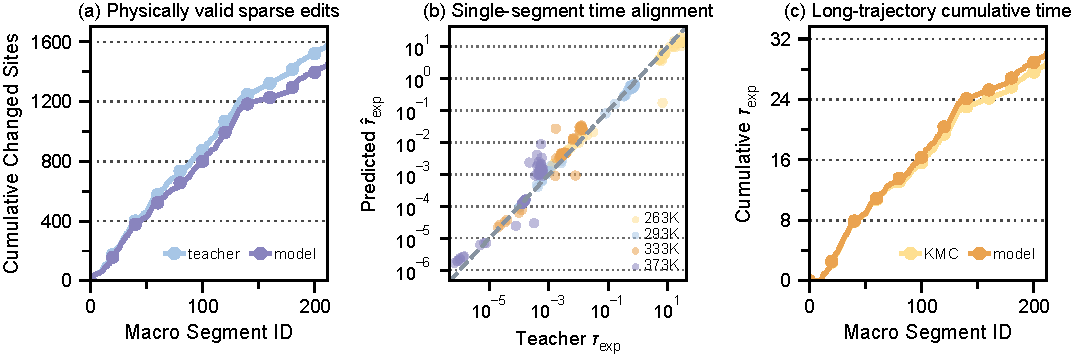
\includegraphics[width=0.88\linewidth,height=0.43\textheight,keepaspectratio]{fig2_main_results.pdf}
  \end{center}
  \vspace{0.08cm}
  \small
  \begin{columns}[T,onlytextwidth]
    \begin{column}{0.58\textwidth}
      \begin{itemize}
        \tightitems
        \item 先在 teacher-supervised segment 上验证单个宏步。
        \item 同时看 sparse edit、projected validity 和 expected-time alignment。
        \item cumulative time trajectory 检查整段宏步时间尺度是否偏移。
      \end{itemize}
    \end{column}
    \begin{column}{0.37\textwidth}
      \hl{Fig.2 证明状态编辑和物理时间可以在同一 segment protocol 下共同对齐。}
    \end{column}
  \end{columns}
\end{frame}

\begin{frame}{实验 2：closed-loop rollout 与消融}
  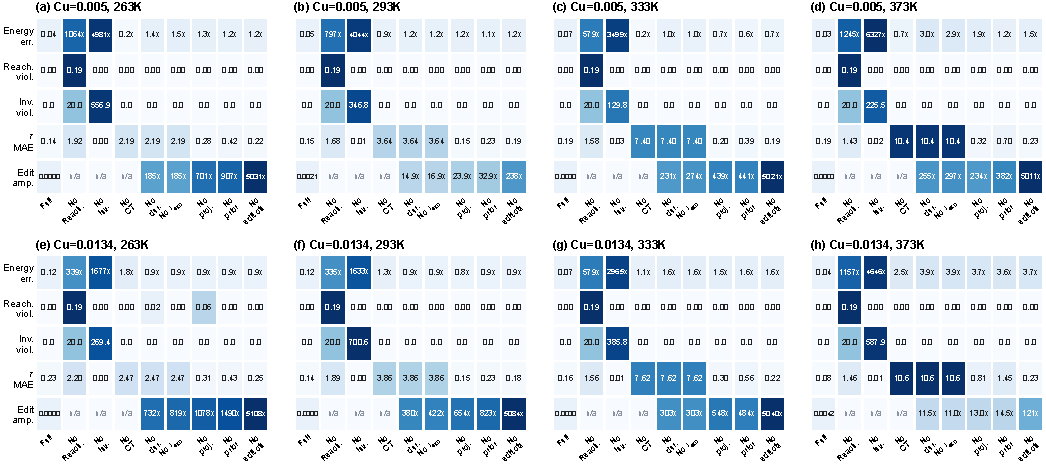
\includegraphics[width=\linewidth,height=0.49\textheight,keepaspectratio]{fig3_closed_loop_results.pdf}
  \vspace{0.05cm}
  \small
  \begin{columns}[T,onlytextwidth]
    \begin{column}{0.48\textwidth}
      \begin{itemize}
        \tightitems
        \item model 消耗自己上一轮的 projected state，形成 autonomous rollout。
      \end{itemize}
    \end{column}
    \begin{column}{0.48\textwidth}
      \begin{itemize}
        \tightitems
        \item teacher probe 只给局部 reference，不覆盖下一步输入。
        \item ablation 分离可达性、库存、duration、projection/prior。
      \end{itemize}
    \end{column}
  \end{columns}
\end{frame}

\begin{frame}{实验 3：长时程诊断与端到端计时}
  \begin{center}
    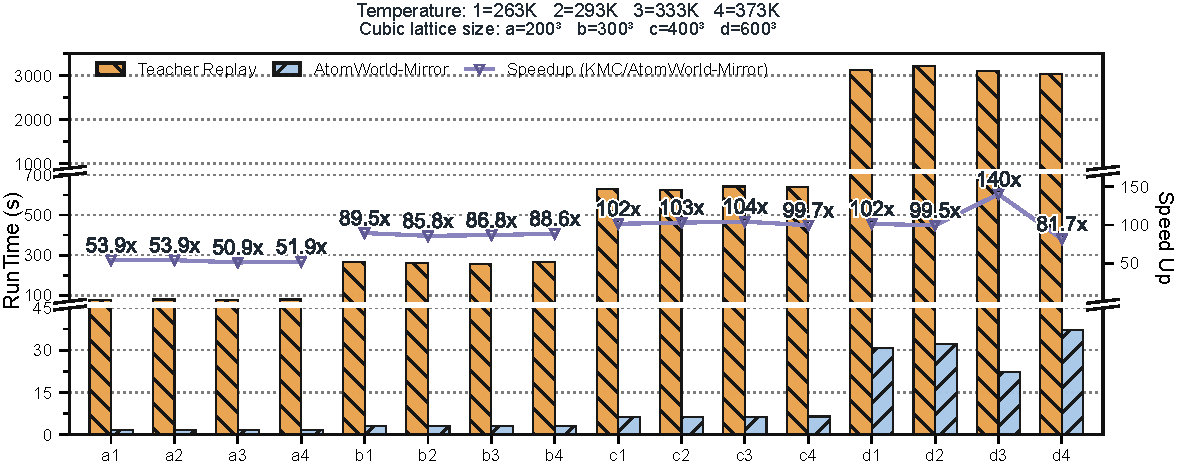
\includegraphics[width=0.86\linewidth,height=0.43\textheight,keepaspectratio]{fig4_speedup_benchmark.pdf}
  \end{center}
  \vspace{0.05cm}
  \small
  \hl{报告口径}
  \vspace{0.05cm}
  \begin{columns}[T,onlytextwidth]
    \begin{column}{0.48\textwidth}
      \begin{itemize}
        \tightitems
        \item 放在 paired 和 closed-loop validity 之后报告。
        \item 端到端计时覆盖 lattice size 与 temperature。
      \end{itemize}
    \end{column}
    \begin{column}{0.48\textwidth}
      \begin{itemize}
        \tightitems
        \item teacher-forced 长轨迹用来隔离时间尺度和 reward 校准。
        \item 不是单独的 neural throughput 数字。
      \end{itemize}
    \end{column}
  \end{columns}
  \framecite{速度必须放在 reachable / inventory-preserving / temporally calibrated 之后解释。}
\end{frame}

\begin{frame}{与已有路线的区别}
  \small
  \begin{tabularx}{\linewidth}{@{}p{0.23\linewidth}X X@{}}
    \toprule
    \textbf{路线} & \textbf{通常优化什么} & \textbf{AtomWorld-Mirror 的区别} \\
    \midrule
    coarse-graining / MSM &
    选择粗变量或 metastable states &
    学习未来相关的 backbone transition，而不是事后聚类 \\
    learned potentials / graph simulators &
    forces、energies、dense next-state dynamics &
    预测 reachable sparse edit + accumulated physical duration \\
    rare-event / policy-guided search &
    让事件遍历更便宜或更偏向目标 &
    保留 rate-governed teacher 的 state-time supervision \\
    \bottomrule
  \end{tabularx}
  \vspace{0.6cm}

  \normalsize
  \hl{定位：}速度提升来自重新设计 atomistic dynamics 的预测表示，而不只是优化某个 simulator 的事件遍历。
\end{frame}

\begin{frame}{总结}
  \begin{columns}[T,onlytextwidth]
    \begin{column}{0.50\textwidth}
      \textbf{中心论点}
      \begin{itemize}
        \tightitems
        \item 长时程材料模拟的瓶颈既是计算成本，也是演化表示。
        \item 逐微事件回放分辨率高，但不等于关键演化分辨率。
        \item 宏步预测必须同时保住状态变化和物理时间。
      \end{itemize}
    \end{column}
    \begin{column}{0.46\textwidth}
      \textbf{方法贡献}
      \begin{itemize}
        \tightitems
        \item 局部可达的稀疏编辑
        \item 库存守恒的投影闭环
        \item 路径条件的物理时间
        \item Multi-K 潜在想象展开
      \end{itemize}
    \end{column}
  \end{columns}
  \vspace{0.7cm}
  \begin{center}
    \large \hl{世界模型加速 = 压缩低影响分辨率，保留有效状态-时间语义。}
  \end{center}
\end{frame}

\begin{frame}{讨论与下一步}
  \begin{columns}[T,onlytextwidth]
    \begin{column}{0.48\textwidth}
      \textbf{当前边界}
      \begin{itemize}
        \tightitems
        \item 受控二元 Fe--Cu 体系
        \item 受控 Multi-K 宏步跨度
        \item 教师探针 / 教师强制诊断
        \item 不是任意关键状态发现系统
      \end{itemize}
    \end{column}
    \begin{column}{0.48\textwidth}
      \textbf{下一步方向}
      \begin{itemize}
        \tightitems
        \item 自然教师模型训练
        \item 其他更复杂体系的模拟
        \item 端到端加速优化
      \end{itemize}
    \end{column}
  \end{columns}
  \vspace{0.9cm}
  \begin{center}
    {\Large 谢谢}
  \end{center}
\end{frame}

\end{document}
